\documentclass{beamer}
\usepackage{graphicx}
\usepackage{amsmath}
\usepackage{subfig}
\usepackage{listings}
\usepackage{tcolorbox,fancyvrb,xcolor,tikz}
\tcbuselibrary{skins,breakable}

\newenvironment{VerbatimIN}
 {\VerbatimEnvironment
  \begin{tcolorbox}[
    breakable,
    colback=lightgray,
    spartan
  ]%
  \begin{Verbatim}}
 {\end{Verbatim}\end{tcolorbox}}

 \newenvironment{VerbatimOUT}
 {\VerbatimEnvironment
  \begin{tcolorbox}[
    breakable,
    spartan
  ]%
  \begin{Verbatim}}
 {\end{Verbatim}\end{tcolorbox}}
 
% Set theme and colors
\usecolortheme{default}

% Set font family and other configurations
% \usepackage{lmodern}
% \renewcommand{\familydefault}{\sfdefault}
% \setbeamertemplate{navigation symbols}{}

\title{Mixed Effects Models - Day 3}
\subtitle{Refreshing Linear Models II}
\author{Marieke Wesselkamp \\ Department of Biometry and Environmental Systems Analysis \\ Albert-Ludwigs-University of Freiburg (Germany)}
\date{February 2023}

\begin{document}

\begin{frame}
  \titlepage
\end{frame}

\begin{frame}{Recap Yesterday}
  \textbf{The relationship between a \textit{continuous} predictor variable and a continuous response variable...}
  
  \begin{figure}[h]
    \centering
    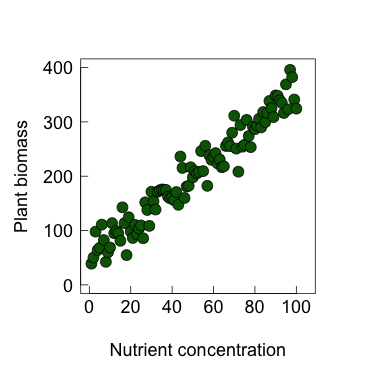
\includegraphics[width=0.5\textwidth]{lectures/day_3_LM_refresh_II/figures/unnamed-chunk-2-1.png} 
    \caption{Scatterplot of nutrient concentration vs. plant biomass.}
  \end{figure}
\end{frame}

\begin{frame}
  \frametitle{}
  \textbf{...can be described by this \textit{model}:}
  
  \begin{equation*}
  y = \beta_0 + \beta_1 \cdot x + \epsilon
  \end{equation*}
  
  \begin{figure}[h]
    \centering
    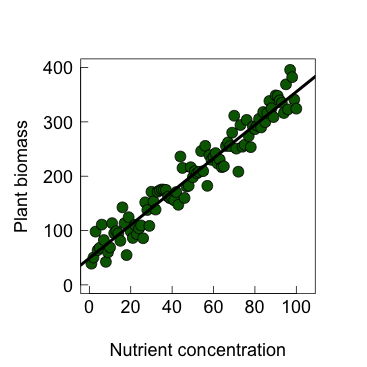
\includegraphics[width=0.5\textwidth]{lectures/day_3_LM_refresh_II/figures/unnamed-chunk-3-1.png} 
    \caption{Linear model fit to the data.}
  \end{figure}
\end{frame}

\begin{frame}
  \frametitle{Matrix Notation}
  \textbf{In matrix notation:}
  
  \begin{equation*}
  \mathbf{y} = \mathbf{X} \cdot \mathbf{\beta} + \mathbf{e}, \quad \epsilon_{iid} \sim \mathcal{N}(0, \sigma^2_{\epsilon} \cdot \mathbf{I})
  \end{equation*}
  where $\mathbf{y}$ are the measured response values, $\mathbf{X}$ is the Design matrix, $\mathbf{\beta}$ is a vector of model parameters, $\mathbf{e}$ is a vector of the errors $\epsilon$, and $\sigma^2_{\epsilon} \cdot \mathbf{I}$ is the variance-covariance matrix of the errors.
\end{frame}

\begin{frame}
  \frametitle{}
  \textbf{The variance-covariance matrix of the \textit{errors}...}

  with $\epsilon_{iid} \sim \mathcal{N}(0, \sigma^2_{\epsilon} \cdot \mathbf{I})$:
  \vspace{0.5cm}
  
  \begin{equation*}
  \scriptsize{\left( \begin{array}{ccccc} 1.52 & 0 & 0 & 0 & 0 \\ 0 & 1.52 & 0 & 0 & 0 \\ 0 & 0 & 1.52 & 0 & 0 \\ 0 & 0 & 0 & 1.52 & 0 \\ 0 & 0 & 0 & 0 & 1.52 \end{array}\right)}
  \end{equation*}
 \vspace{0.5cm}
 
  \begin{itemize}
    \item \textbf{Note:} The variances are on the diagonals, and the covariances are on the off-diagonals.
  \end{itemize}
\end{frame}

\begin{frame}[fragile]
  \frametitle{}
  \begin{columns}
      \begin{column}{0.42\textwidth}
        \textbf{...is not the variance-covariance matrix of the \textit{parameters}.}
        \tiny
        \begin{VerbatimIN}[numbers=left,numbersep=6pt]
vcov(mod)
        \end{VerbatimIN}
        \begin{VerbatimOUT}[numbers=left,numbersep=6pt]
            (Intercept)          x
(Intercept)   2.4675458 -0.9213982
x            -0.9213982  0.3922764



cov2cor(vcov(mod)) 
# turned into correlations

            (Intercept)          x

(Intercept)   1.0000000 -0.9365234
x            -0.9365234  1.0000000
        \end{VerbatimOUT}
      \end{column}
      \begin{column}{0.58\textwidth}
      \tiny
          \begin{VerbatimOUT}[numbers=left,numbersep=6pt]
Call:
lm(formula = y ~ x)

Residuals:
      1       2       3       4       5 
-0.6903  0.9505  0.5261 -1.5298  0.7435 

Coefficients:
            Estimate Std. Error t value Pr(>|t|)  
(Intercept)  -1.4403     1.5708  -0.917   0.4268  
x             3.2661     0.6263   5.215   0.0137 *
---
Signif. codes:  0 '***' 0.001 '**' 0.01 '*' 0.05 
'.' 0.1 ' ' 1

Residual standard error:     
1.232 on 3 degrees of freedom
Multiple R-squared:  0.9006,    
Adjusted R-squared:  0.8675 
F-statistic: 27.19 on 1 and 3 DF,  
p-value: 0.01371

Correlation of Coefficients:
  (Intercept)
x -0.94    
          \end{VerbatimOUT}
      \end{column}
  \end{columns}

 %The variance-covariance matrix of parameters is different and involves correlations among the model parameters.

\end{frame}

\begin{frame}
  \frametitle{}
  \begin{center}
    \huge\textbf{\textcolor{purple}{Categorical predictors}}
  \end{center}
\end{frame}

\begin{frame}
  \frametitle{}
  \textbf{The design matrix for a continuous predictor:}

  \begin{equation*}
  \mathbf{x} = \left( \begin{array}{cc} 1 & x_{1} \\ 1 & x_{2} \\ . & . \\ . & . \\ . & . \\ 1 & x_{n-1} \\ 1 & x_n \end{array}\right)
  \end{equation*}

  with 1's for the intercept and a column with the actual x-values.
\end{frame}

\begin{frame}
  \frametitle{}
  \textbf{What if there are only two values of a predictor with several measurements of the response at these values?*}

  \begin{itemize}
    \item \textbf{Note:} This is \textit{NOT} grouping as long as the measurements taken at the same predictor value are from \textit{different} units.
  \end{itemize}
  
  \begin{figure}[h]
    \centering
    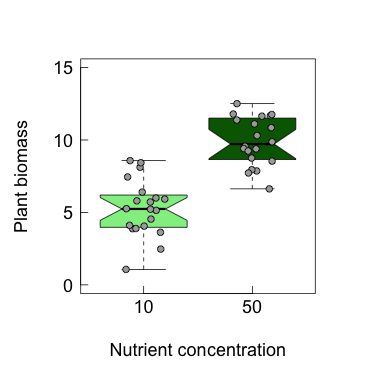
\includegraphics[width=0.5\textwidth]{lectures/day_3_LM_refresh_II/figures/unnamed-chunk-8-1.png} 
    \caption{Boxplot of response by nutrient concentration.}
  \end{figure}
\end{frame}

\begin{frame}
  \frametitle{}
  \textbf{The question is now usually not how the response increases with the predictor, but what the \textit{difference} in the response between the low and high values of the predictor is.}
  
  \begin{figure}[h]
    \centering
    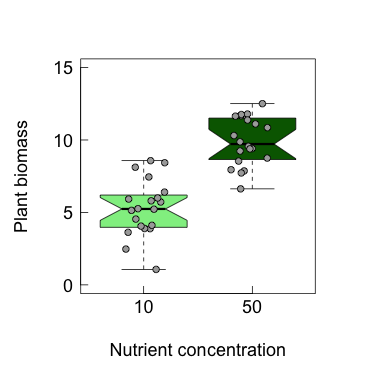
\includegraphics[width=0.5\textwidth]{lectures/day_3_LM_refresh_II/figures/unnamed-chunk-9-1.png} 
    \caption{Difference in response by nutrient concentration.}
  \end{figure}
\end{frame}

\begin{frame}
  \frametitle{}
  \textbf{The matrix notation is identical...}

  \begin{equation*}
  \mathbf{y} = \mathbf{X} \cdot \mathbf{b} + \mathbf{e}, \quad \epsilon \sim \mathcal{N}(0, \sigma^2_{\epsilon} \cdot \mathbf{I})
  \end{equation*}
\end{frame}

\begin{frame}
  \frametitle{}
  \textbf{...but the design matrix for a \textit{categorical} predictor looks different:}

  \begin{equation*}
  \tiny {\mathbf{x} = \left( \begin{array}{cc} 1 & 0 \\ 1 & 0 \\ 1 & 0 \\ . & . \\ . & . \\ 1 & 1 \\ 1 & 1 \\ 1 & 1 \end{array}\right) }
  \end{equation*}
  
  The categorical (here: binary) variable is encoded as 0 and 1, regardless of its content. This is a \textit{dummy variable} that takes 0 for the first and 1 for the second treatment level.
\end{frame}

\begin{frame}
  \frametitle{}
  \textbf{This changes the interpretation of our linear model parameters:}

  \begin{equation*}
  y = \beta_0 + \beta_1 \cdot x + \epsilon
  \end{equation*}
  
  What happens when $x$ is 0?
  
  \begin{equation*}
  y = \beta_0 + \beta_1 \cdot 0 + \epsilon = \beta_0 + \epsilon
  \end{equation*}
  
  $\beta_0$ now represents the mean of the first treatment, and $\beta_1$ the difference of the second treatment to that mean.
  
  \begin{figure}[h]
    \centering
    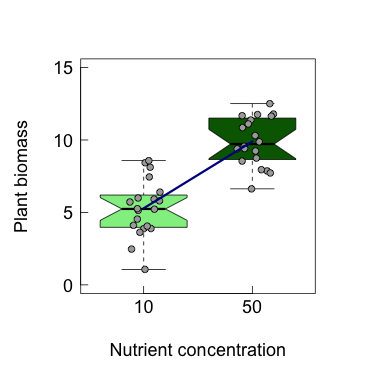
\includegraphics[width=0.5\textwidth]{lectures/day_3_LM_refresh_II/figures/unnamed-chunk-10-1.png} 
    \caption{Interpretation of model parameters.}
  \end{figure}
\end{frame}

\begin{frame}
  \frametitle{}
  \textbf{Accordingly, multiple levels are encoded into multiple dummy variables.}
  
  \begin{figure}[h]
    \centering
    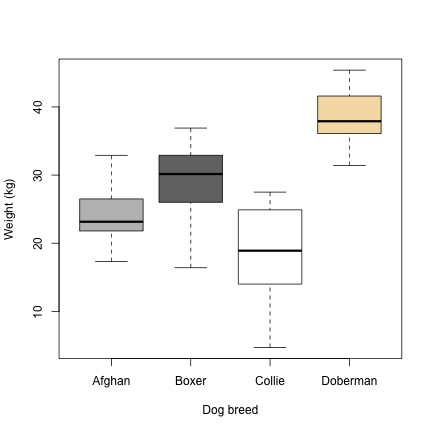
\includegraphics[width=0.6\textwidth]{lectures/day_3_LM_refresh_II/figures/unnamed-chunk-12-1.png} 
    \caption{Boxplot of dog weights by breed.}
  \end{figure}
\end{frame}

\begin{frame}
  \frametitle{}
  \textbf{With k categories, there are k-1 dummy variables, each representing a unique category.}
  \vspace{0.5cm}
  
  \begin{equation*}
  \tiny {\mathbf{x} = \left( \begin{array}{cccc} 1 & 0 & 0 & 0 \\ 1 & 0 & 0 & 0 \\ 1 & 1 & 0 & 0 \\ 1 & 1 & 0 & 0 \\ 1 & 0 & 1 & 0 \\ 1 & 0 & 1 & 0 \\ 1 & 0 & 0 & 1\\ 1 & 0 & 0 & 1 \end{array}\right) }
  \end{equation*}
  \vspace{0.5cm}

  with the first column of 1's for the first mean and the other columns of 0's and 1's for the \textit{differences} to that baseline.
\end{frame}

\begin{frame}
  \frametitle{}
  \begin{figure}[h]
    \centering
    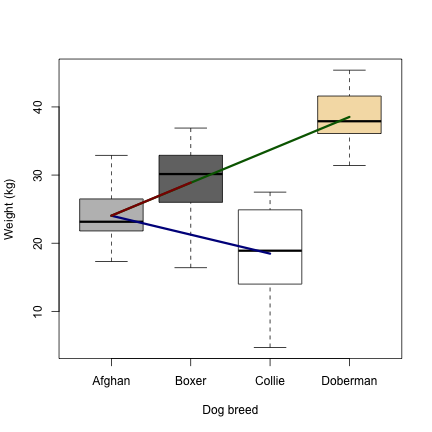
\includegraphics[width=0.6\textwidth]{lectures/day_3_LM_refresh_II/figures/unnamed-chunk-13-1.png} 
    \caption{Differences between breeds.}
  \end{figure}
\end{frame}

\begin{frame}[fragile]
  \frametitle{Analysis of variance with a binary predictor}
  \scriptsize
  \begin{VerbatimIN}[numbers=left,numbersep=6pt]
model.aov <- aov(y ~ x, ex)
  \end{VerbatimIN}
 \begin{VerbatimOUT}[numbers=left,numbersep=6pt]
summary(model.aov)


            Df Sum Sq Mean Sq F value   Pr(>F)    
x            1  212.9  212.91   65.12 9.24e-10 ***
Residuals   38  124.2    3.27                     
---
Signif. codes:  0 '***' 0.001 '**' 0.01 '*' 0.05 '.' 0.1 ' ' 1
 \end{VerbatimOUT}


  
\end{frame}

\begin{frame}
  \frametitle{ANOVA Table}

  \resizebox{\linewidth}{!}{
  \begin{tabular}{lccccc}
    Source & SS & df & MS & F & p \\
    \hline
    Treatment & SS$_{Treat}$ & k$_{Treat}$ - 1 & SS$_{Treat}$ / df$_{Treat}$ & MS$_{Treat}$ / MS$_{Res}$ \\
    Residual & SS$_{Res}$  & N - k & SS$_{Res}$ / df$_{Res}$ \\
    Total & SS$_{Total}$ & N - 1 \\
  \end{tabular}}
  
  \vspace{1cm}
  \begin{equation*}
  Variance_{total} = Variance_{treatment} + Variance_{residual}
  \end{equation*}
\end{frame}

\begin{frame}[fragile]
  \frametitle{}
  \textbf{aov()} focuses on hypothesis tests, less on parameter estimation.
  \scriptsize
  \begin{VerbatimIN}[numbers=left,numbersep=6pt]
coef(model.aov) # to get the parameter values
  \end{VerbatimIN}
  \begin{VerbatimOUT}[numbers=left,numbersep=6pt]
(Intercept)         x50 
   5.283248    4.614238 
  \end{VerbatimOUT}
  \begin{VerbatimIN}[numbers=left,numbersep=6pt]
model.tables(model.aov, type = "means", se = TRUE) # alternative
  \end{VerbatimIN}
  \begin{VerbatimOUT}[numbers=left,numbersep=6pt]
Tables of means
Grand mean

7.590367 

 x 
x
   10    50 
5.283 9.897 

Standard errors for differences of means
             x
        0.5718
replic.     20      
  \end{VerbatimOUT}



\end{frame}

\begin{frame}[fragile]
  \frametitle{}
  \textbf{lm()} and \textbf{aov()} give the same results but in different formats.
  \scriptsize
  \begin{VerbatimIN}[numbers=left,numbersep=6pt]
model.lm <- lm(y ~ x, ex)
summary(model.lm)      
  \end{VerbatimIN}
  \begin{VerbatimOUT}[numbers=left,numbersep=6pt]
Call:
lm(formula = y ~ x, data = ex)

Residuals:
    Min      1Q  Median      3Q     Max 
-4.2165 -1.2604 -0.0433  1.2777  3.2906 

Coefficients:
            Estimate Std. Error t value Pr(>|t|)    
(Intercept)   5.2832     0.4043  13.066 1.24e-15 ***
x50           4.6142     0.5718   8.069 9.24e-10 ***
---
Signif. codes:  0 '***' 0.001 '**' 0.01 '*' 0.05 '.' 0.1 ' ' 1

Residual standard error: 1.808 on 38 degrees of freedom
Multiple R-squared:  0.6315,    Adjusted R-squared:  0.6218 
F-statistic: 65.12 on 1 and 38 DF,  p-value: 9.239e-10
  \end{VerbatimOUT}
\end{frame}

\begin{frame}{}
  \begin{center}
    \huge\textbf{\textcolor{purple}{Multiple predictors}}
  \end{center}
\end{frame}

\begin{frame}{Multivariate Regression}
  As soon as we have more than two predictors:
  
  \begin{itemize}
      \item \texttt{lm(y \textasciitilde{} x.1 + x.2 + ... + x.n,...)}
  \end{itemize}
  \vspace{0.5cm}
  
  The \textbf{deterministic part} requires \textit{at least} n + 1 coefficients:
  
  \begin{equation*}
    \mathbf{y} = \beta_0 + \beta_1 \cdot x_1 + \beta_2 \cdot x_2 + ... + \beta_n \cdot x_n 
  \end{equation*}
\end{frame}

\begin{frame}
  \frametitle{}
  Predictors can be only categorical, only continuous, or a mixture of both.
  \vspace{0.5cm}
  \begin{table}[h]
    \centering
    \begin{tabular}{ccc}
      \hline
      $\mathbf{y}$ & $x_1$ & $x_2$ \\
      \hline
      3.32 & 1.0 & control \\
      4.32 & 2.3 & control \\
      2.09 & 4.2 & control \\
      . & . & . \\
      . & . & . \\
      2.12 & 2.0 & treatment \\
      4.02 & 4.1 & treatment \\
      8.12 & 5.4 & treatment \\
      \hline
    \end{tabular}
  \end{table}
\end{frame}

\begin{frame}
  \frametitle{}
  Exemplary design matrix for one continuous and one binary predictor:
  
  \begin{equation*}
  \mathbf{x} = \left( \begin{array}{ccc} 1 & x_{1} & 0 \\ 1 & x_{2} & 0 \\ 1 & x_{3} & 0 \\ . & . & . \\ . & . & . \\ 1 & x_{n-2} & 1 \\ 1 & x_{n-1} & 1 \\ 1 & x_n & 1 \end{array}\right)
  \end{equation*}
\end{frame}

\begin{frame}[fragile]
  \frametitle{}
  \begin{columns}
      \begin{column}{0.5\textwidth}
        \textbf{Why not simply use two univariate models, one per predictor?}
        \vspace{0.5cm}
        
        \texttt{lung capacity} \textit{may} depend on \texttt{smoking} and \texttt{age}.
      \end{column}
      \begin{column}{0.5\textwidth}
      \scriptsize
      \begin{VerbatimIN}
    LungCap Age Smoke
1     6.475   6    no
2    10.125  18   yes
3     9.550  16    no
4    11.125  14    no
5     4.800   5    no
6     6.225  11    no
      \end{VerbatimIN}
      \begin{VerbatimIN}
    LungCap Age Smoke
720   7.325   9    no
721   5.725   9    no
722   9.050  18   yes
723   3.850  11   yes
724   9.825  15    no
725   7.100  10    no          
      \end{VerbatimIN}
      \end{column}
  \end{columns}
\end{frame}

\begin{frame}[fragile]
  \frametitle{}
  \begin{columns}
      \begin{column}{0.5\textwidth}
        \textbf{First univariate model:} smoking increases lung capacity by nearly a liter.
        \vspace{0.3cm}
        
        \textit{Really? Should all professional athletes smoke a pack or two a day now?}
        \vspace{0.5cm}
        
        \scriptsize
        \begin{VerbatimOUT}[numbers=left,numbersep=6pt]
Estimate Std. Error
(Intercept)     7.77       0.10
Smokeyes        0.88       0.32      
        \end{VerbatimOUT}
      \end{column}
      \begin{column}{0.5\textwidth}
      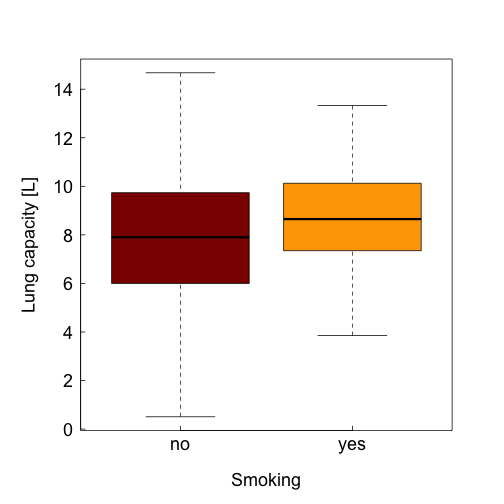
\includegraphics[width=\textwidth]{lectures/day_3_LM_refresh_II/figures/unnamed-chunk-21-1.png}
      \end{column}
  \end{columns}   
\end{frame}

\begin{frame}[fragile]
  \frametitle{}
    \begin{columns}
      \begin{column}{0.5\textwidth}
        \textbf{Second univariate model:} \\
        aging increases lung capacity by half a liter every year
        \vspace{0.3cm}

        \textit{A body growth effect}
      \vspace{0.5cm}

      \scriptsize
      \begin{VerbatimOUT}[numbers=left,numbersep=6pt]
            Estimate Std. Error
(Intercept)     1.15       0.18
Age             0.54       0.01
      \end{VerbatimOUT}
      \end{column}
      \begin{column}{0.5\textwidth}
      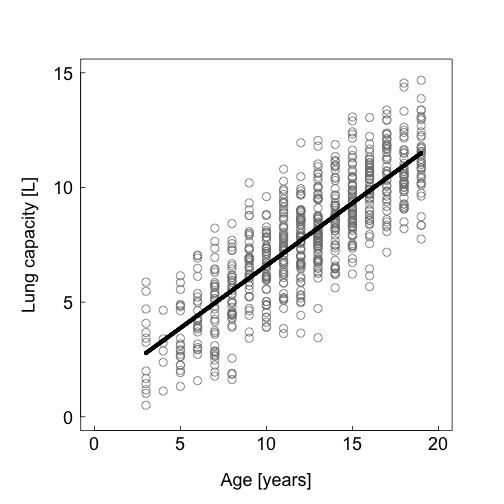
\includegraphics[width=\textwidth]{lectures/day_3_LM_refresh_II/figures/unnamed-chunk-23-1.png}
      \end{column}
  \end{columns}  
\end{frame}

\begin{frame}[fragile]
  \frametitle{}
    \begin{columns}
      \begin{column}{0.5\textwidth}
        Smoking and Age are correlated = confounded.\\
        \textit{Children (hopefully) don't smoke but have small lungs.}
        \vspace{0.5cm}

        \scriptsize
        \begin{VerbatimIN}[numbers=left,numbersep=6pt]
library(psych)
biserial(lung$Age, lung$Smoke)
        \end{VerbatimIN}
        \begin{VerbatimOUT}[numbers=left,numbersep=6pt]
          [,1]
[1,] 0.3547211            
        \end{VerbatimOUT}
      \end{column}
      \begin{column}{0.5\textwidth}
      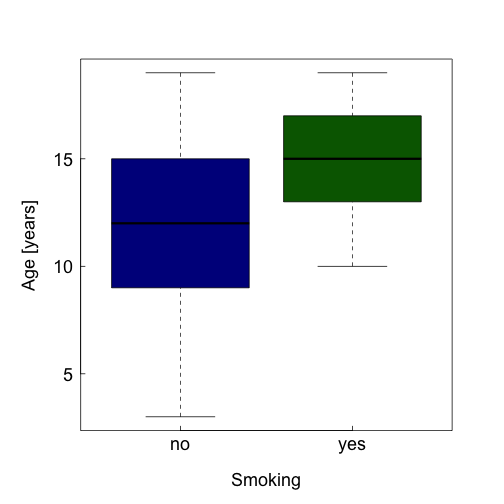
\includegraphics[width=\textwidth]{lectures/day_3_LM_refresh_II/figures/unnamed-chunk-25-1.png}
      \end{column}
  \end{columns} 
  \vspace{1cm}
  
  \tiny{* biserial correlations are between a continuous and a categorical random variable}
\end{frame}

\begin{frame}[fragile]
  \frametitle{Now a multivariate model}
  \begin{columns}
      \begin{column}{0.5\textwidth}
      \scriptsize
      \begin{VerbatimIN}[numbers=left,numbersep=6pt]
m <- glm(LungCap ~ Age + Smoke, 
         data = lung)          
      \end{VerbatimIN}
      \begin{VerbatimOUT}[numbers=left,numbersep=6pt]
            Estimate Std. Error
(Intercept)     1.09       0.18
Age             0.56       0.01
Smokeyes       -0.65       0.19
      \end{VerbatimOUT}
      \vspace{0.3cm}
      
      \normalsize\textbf{Indeed, smoking decreases lung capacity by 0.65 liter}
      \end{column}
      \begin{column}{0.5\textwidth}
        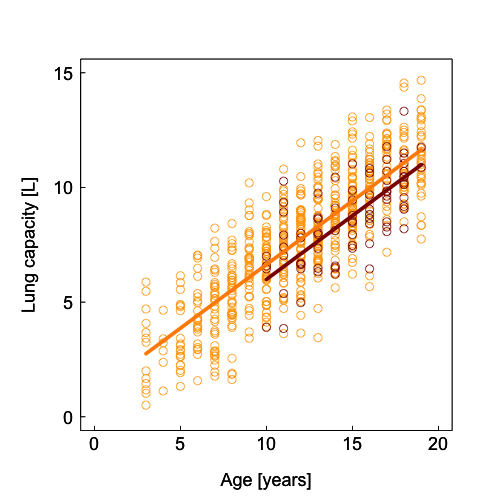
\includegraphics[width=\textwidth]{lectures/day_3_LM_refresh_II/figures/unnamed-chunk-28-1.png}
      \end{column}
  \end{columns}
\end{frame}

\begin{frame}[fragile]
\frametitle{Predictions}
    \begin{columns}
        \begin{column}{0.5\textwidth}
          A 15-year-old \textbf{smoker} has an expected lung capacity of:
          \begin{equation*}
          1.09 + 0.56 \cdot 15 - 1 \cdot 0.65 = 8.84 \text{ liters}
          \end{equation*}
          \vspace{0.3cm}
          
          A 15-year-old \textbf{non-smoker} has an expected lung capacity of:
          \begin{equation*}
          1.09 + 0.56 \cdot 15 - 0 \cdot 0.65 = 9.49 \text{ liters}
          \end{equation*}
        \end{column}
        \begin{column}{0.5\textwidth}
            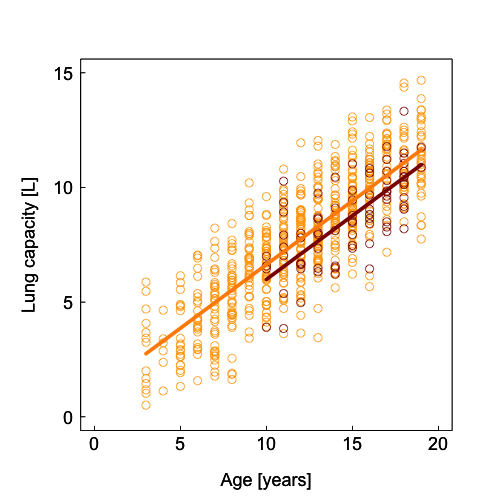
\includegraphics[width=\textwidth]{lectures/day_3_LM_refresh_II/figures/unnamed-chunk-28-1.png}
            \scriptsize
            \begin{VerbatimOUT}[numbers=left,numbersep=6pt]
            Estimate Std. Error
(Intercept)     1.09       0.18
Age             0.56       0.01
Smokeyes       -0.65       0.19
            \end{VerbatimOUT}
        \end{column}
    \end{columns}
\end{frame}

\begin{frame}
  \frametitle{Reasons for Multivariate Regression}
  \begin{itemize}
    \item Multiple causation
    \item Statistical control for confounds
    \item Interaction
  \end{itemize}
\end{frame}

\begin{frame}
    \centering
    \huge\color{purple}\textbf{Break!}
\end{frame}

\begin{frame}
  \frametitle{Omitted Variable Bias}
  \textbf{Missing predictors distort the regression outcome when:}
  \begin{itemize}
    \item They influence the response.
    \item \textbf{AND} they are correlated with an included predictor.
  \end{itemize}

\vspace{0.5cm}
  
  \begin{block}{}
  \centering
    \large\textbf{Omitted Variable Bias} (OVB)
  \end{block}
\end{frame}

\begin{frame}
  \frametitle{}
\begin{tabular}{cl}
   \begin{tabular}{c}
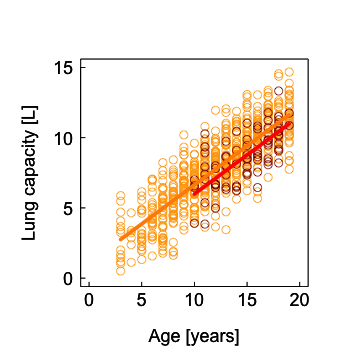
\includegraphics[width=0.5\textwidth]{lectures/day_3_LM_refresh_II/figures/unnamed-chunk-31-1.png}
   \end{tabular}
   &
   \begin{tabular}{l}
       \parbox{0.4\linewidth}{
         When predictors are correlated \textbf{and} both influence the response, multivariate regression prevents the \textbf{omitted variable bias}!
        }
   \end{tabular}
 \end{tabular}
\end{frame}

\begin{frame}
    \frametitle{}
    \textbf{BUT}, imagine $x_1$ fully correlates with $x_2$ so that e.g.: $x_2 = 2 * x_1$ Then:
    \begin{equation*}
        \begin{aligned}
        y = 5 + 2 * x_1 + 1 * x_2 \\
        \textit{or } y = 5 + 2 * x_2 \\
        \textit{or } y = 5 + 4 * x_1 \\
        \textit{ etc. ...}
        \end{aligned}
    \end{equation*}
    \vspace{0.5cm}
    
    The Log-Likelihood can be equally high for different combinations of the coefficients for $x_2$ and $x_2$\\
    \textbf{= bad estimates and high standard errors}
\end{frame}

\begin{frame}
  \frametitle{}
  \textbf{Correlated predictors make it difficult to estimate coefficients because of \textit{variance inflation}.}
  \\
  Remember the variance estimation for the linear coefficient:
  \begin{equation*}
      cov(\hat{\beta}_j) = \sigma(\textbf{X'X})^{-1}
  \end{equation*}

  This can be reformulated to:
  
  \begin{equation*}
    Var(\hat{\beta}_j) = \frac{1}{(1-R^2)} \cdot \frac{\sigma^2}{\sum_{i=1}^{n} (x_{ij} - \overline{x}_j)^2}
  \end{equation*}
  
  A small model variance $\sigma^2$ and a small $R^2$ lead to small variances of $\hat{\beta}$.
\end{frame}

\begin{frame}[fragile]
    \frametitle{In R}
    \scriptsize
    \begin{VerbatimIN}[numbers=left,numbersep=6pt]
set.seed(123)
n = 20 
x1 <- runif(n, 0, 10)
x2 <- 0.5 * x1 + rnorm(n, 0, 0.5)

cor(x1, x2)        
    \end{VerbatimIN}
    \begin{VerbatimOUT}[numbers=left,numbersep=6pt]
[1] 0.9467951        
    \end{VerbatimOUT}
    \begin{VerbatimIN}[numbers=left,numbersep=6pt]
y <- rnorm(n, mean = 0 + 0.25 * x1 + 0.75 * x2, sd = 1)
fm <- glm(y ~ x1 + x2 -1)        
    \end{VerbatimIN}
    \begin{VerbatimOUT}[numbers=left,numbersep=6pt]
   Estimate Std. Error
x1     0.12       0.20
x2     1.03       0.41        
    \end{VerbatimOUT}

    \normalsize\textbf{Not close to 0.25 and 075}
\end{frame}

\begin{frame}
    \frametitle{We have a dilemma...}
    \large{Too few correlated predictors distort results \textbf{(the omitted variable bias)}, but too many correlated predictors can, too \textbf{(variance inflation)}.}
\end{frame}

\begin{frame}
  \frametitle{Variance - Bias Trade-off}
  \textbf{The problem of minimizing two sources of errors.}
  
  \begin{itemize}
    \item Either high explained variance but low generality (\textit{overfitting the data}).
    \item Or low bias (high general insights) but lower fit to the specific data.
  \end{itemize}
  
  \begin{center}
    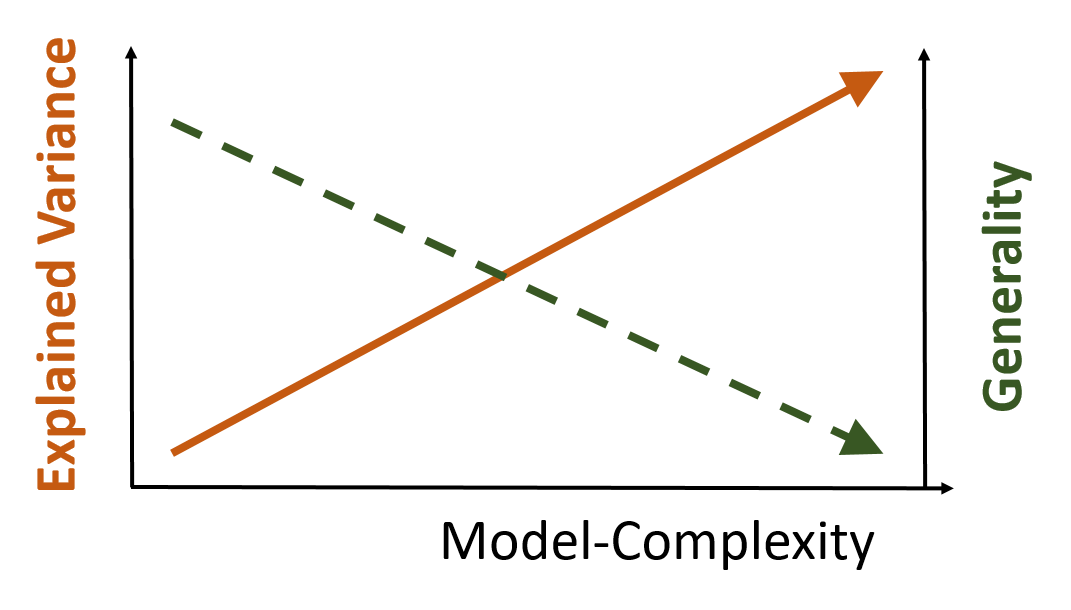
\includegraphics[width=0.85\textwidth]{figures/var-bias-tradeoff.png} 
  \end{center}
\end{frame}

\begin{frame}
  \frametitle{Overfitting}
  \textbf{Too many predictors can cause \textit{Overfitting}.}
  
  \begin{itemize}
    \item A model overfits the data when it re-draws the specifics of the dataset but doesn't deliver general/transferable insights.
  \end{itemize}
  
  \begin{center}
    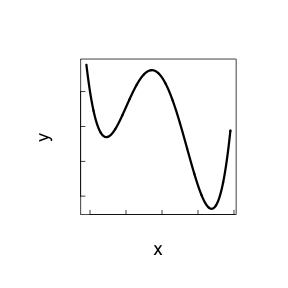
\includegraphics[width=0.6\textwidth]{lectures/day_3_LM_refresh_II/figures/unnamed-chunk-35-1.png} 
  \end{center}
\end{frame}

\begin{frame}
    \frametitle{}   
    \textbf{With increasing degrees of freedom, we increasingly fit the noise in the data.}\\
    \vspace{0.5cm}
        
    \centering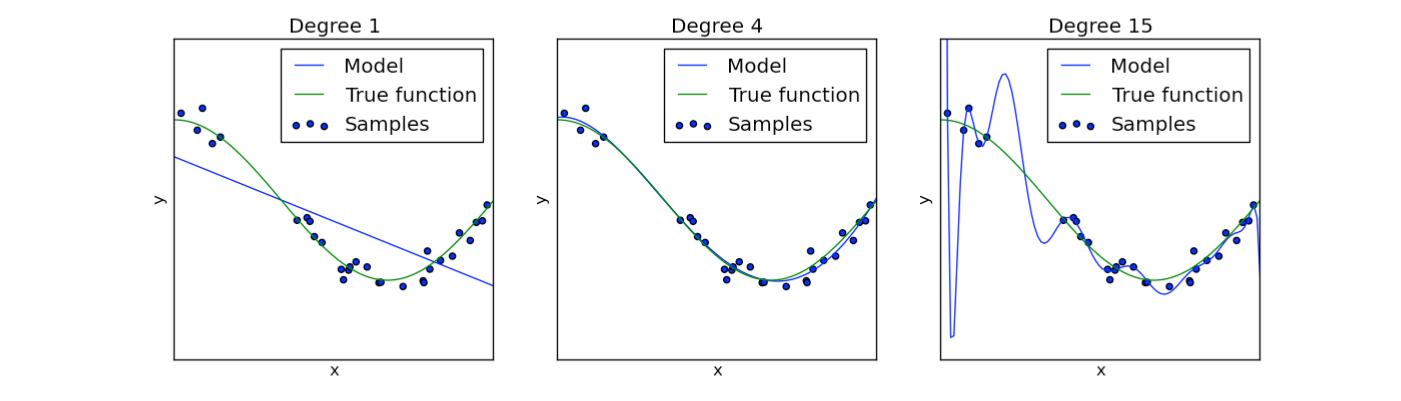
\includegraphics[width=1\textwidth]{lectures/day_3_LM_refresh_II/figures/overfitting.png}
    \vspace{0.5cm}

    \textit{Rule of thumb: 10 data points per model coefficient}
\end{frame}

\begin{frame}{}
  \begin{center}
    \huge\textbf{\textcolor{purple}{Interactions between predictors}}
  \end{center}
\end{frame}

\begin{frame}
  \frametitle{Linear Model Without Interaction}
  \textbf{Additive model}
  
  The two predictors are associated with the response independently of each other.
  
  \begin{equation*}
    y = \beta_0 + \beta_1 \cdot x_1 + \beta_2 \cdot x_2 + \epsilon
  \end{equation*}
\end{frame}

\begin{frame}
  \frametitle{Including an Interaction}
  \textbf{Multiplicative model}
  
  The effect of one predictor on the response depends on the values of another predictor:
  
  \begin{equation*}
    y = \beta_0 + \beta_1 \cdot x_1 + \beta_2 \cdot x_2 + \beta_3 \cdot (x_1 \times x_2) + \epsilon
  \end{equation*}
  
  There is now a third parameter $\beta_3$ for the interaction.
\end{frame}

\begin{frame}
  \frametitle{Interaction...}
  \begin{columns}
      \begin{column}{0.5\textwidth}
      ...between two categorical (binary) predictors:
      \vspace{0.5cm}
      
      $x_1$: Coffee machine ($A$: French press or $B$: De'Longhi)\\
      $x_2$: Coffee type ($1$: Lavazza or $2$: Schwarzwild)\\
      Response: some proxy for taste    
      \end{column}
      \begin{column}{0.5\textwidth}
      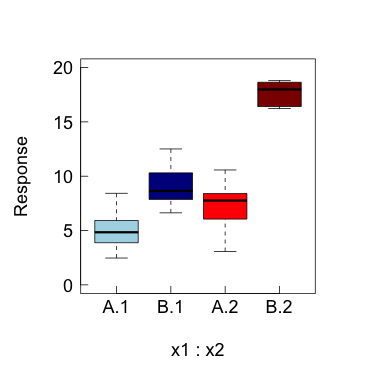
\includegraphics[width=\textwidth]{lectures/day_3_LM_refresh_II/figures/unnamed-chunk-36-1.png}
      \end{column}
  \end{columns}
\end{frame}

\begin{frame}
  \frametitle{Interaction...}
  \begin{columns}
      \begin{column}{0.5\textwidth}
          ...between a categorical and a continuous predictor:
      \vspace{0.5cm}

          $x_1$: Nutrient score (color code)
          $x_2$: Temperature
      \end{column}
      \begin{column}{0.5\textwidth}
      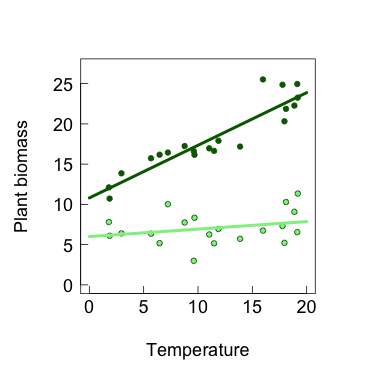
\includegraphics[width=\textwidth]{lectures/day_3_LM_refresh_II/figures/unnamed-chunk-37-1.png}
      \end{column}
  \end{columns}
\end{frame}

\begin{frame}[fragile]
  \frametitle{What do the interaction coefficients tell us?}
  
  \begin{equation*}
    y = \beta_0 + \beta_1 \cdot x_1 + \beta_2 \cdot x_2 + \beta_3 \cdot (x_1 \times x_2) + \epsilon
  \end{equation*}
  \scriptsize
  \begin{VerbatimOUT}[numbers=left,numbersep=6pt]
Call:
lm(formula = y ~ x1 + x2 + x1 * x2, data = ex.2)

Residuals:
    Min      1Q  Median      3Q     Max 
-3.9151 -1.1308 -0.1784  1.1192  4.2320 

Coefficients:
            Estimate Std. Error t value Pr(>|t|)    
(Intercept)  6.00879    0.91601   6.560 1.25e-07 ***
x150         4.83154    1.29543   3.730 0.000658 ***
x2           0.09318    0.07128   1.307 0.199405    
x150:x2      0.56086    0.10080   5.564 2.66e-06 ***
---
Signif. codes:  0 '***' 0.001 '**' 0.01 '*' 0.05 '.' 0.1 ' ' 1

Residual standard error: 1.85 on 36 degrees of freedom
Multiple R-squared:  0.9269,    Adjusted R-squared:  0.9208 
F-statistic: 152.1 on 3 and 36 DF,  p-value: < 2.2e-16
  \end{VerbatimOUT}
\end{frame}

\begin{frame}
    \frametitle{}
    \textbf{More interaction possibilities with one categorical and one continuous predictor:}
    \vspace{0.5cm}

    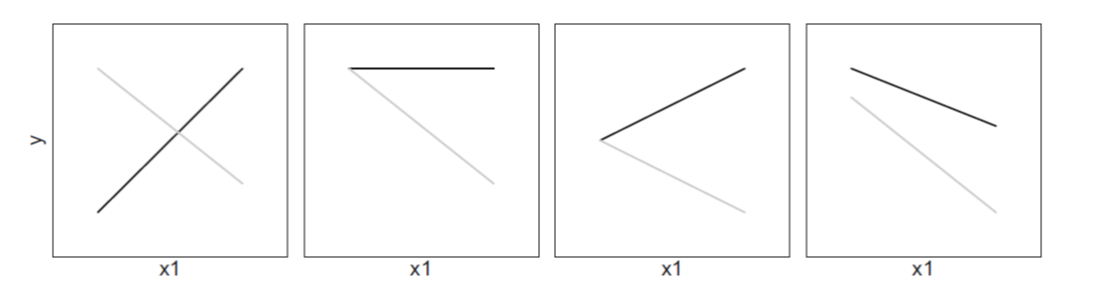
\includegraphics[width=1\textwidth]{lectures/day_3_LM_refresh_II/figures/more_interactions.png}
\end{frame}

\begin{frame}
    \frametitle{These are not interactions:}
    \begin{columns}
        \begin{column}{0.4\textwidth}
            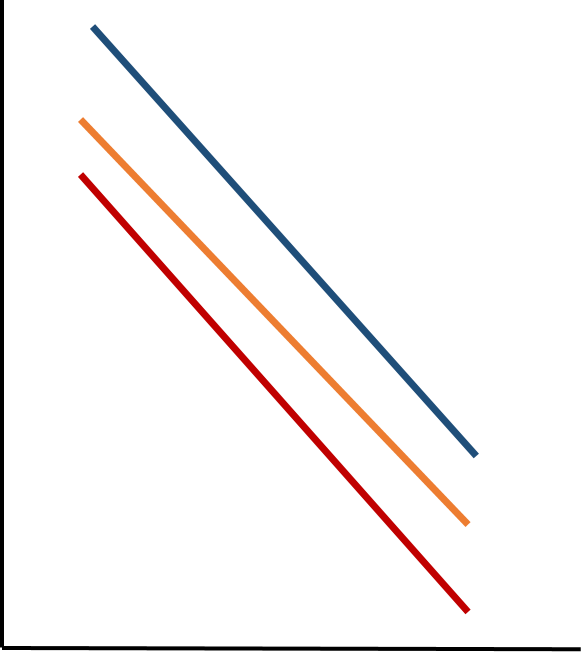
\includegraphics[width=\textwidth]{lectures/day_3_LM_refresh_II/figures/no-inter-1.png}
        \end{column}
        \begin{column}{0.45\textwidth}
            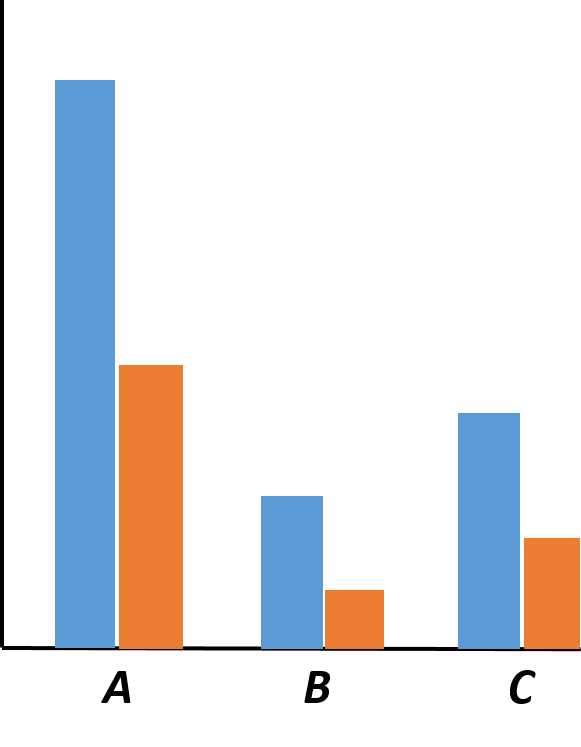
\includegraphics[width=\textwidth]{lectures/day_3_LM_refresh_II/figures/no-inter-2.png}
        \end{column}
    \end{columns}
\end{frame}

\begin{frame}
    \frametitle{}
    \centering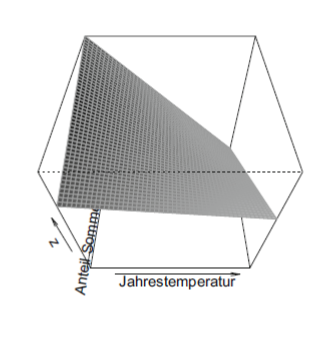
\includegraphics[width=0.7\textwidth]{lectures/day_3_LM_refresh_II/figures/2-cont-interactions.png}
\end{frame}

\begin{frame}
  \frametitle{Recapitulation Day 3}
  After today, you should know and understand:
  \begin{itemize}
    \item What the difference between \textbf{continuous} and \textbf{categorical} predictors is.
    \item How \textbf{multiple} predictors can be included in a statistical model.
    \item What an \textbf{interaction} between predictors is.
    \item What R functions to use.
  \end{itemize}
  
  \vspace{1cm}
  Today afternoon: practical exercises about \textbf{categorical} and \textbf{multiple predictors} and \textbf{interactions} in R.
\end{frame}

\end{document}